\Chapter{Megvalósítás}
\Section{Ütemező módosítása}
A feladat a Linux processz ütemező optimalizálása, különféle használati módokra.
Ehhez módosításokat kell hogy végezzek az ütemezőn, amit megtehetek úgy hogy, konkrétan a forráskódot írom át, ezután újra lefordítom a kernelt és megfigyelem a módosítások hatásait.
A probléma hogy ez a folyamat hosszadalmas lehet, emiatt kerestem más módszereket.
Megfigyeltem hogy a több változó is elérhető az ütemező hangolására, így nincs szükség arra hogy újakat vezessek be.

Ezeket a változókat megtalálhatjuk a /proc/sys/kernel/ jegyzékben, fontos kiemelni hogy ezek a változók futásidőben is módosíthatók. Minden változóhoz tartozik egy intervallum, amin belül tetszőlegesen módosítható az értéke. 

Az értékek módosítását megadhatjuk direkt:
\begin{python}
$ echo $value > /proc/sys/kernel/sched_min_granularity_ns
\end{python}%$

A másik lehetőség, a sysctl interfészen keresztül történő megadás:
\begin{python}
$ sudo sysctl -w sched_latency_ns=VALUE
\end{python}%$
A sysctl interfész segítségével lekérdezhetem, módosíthatom a kernel változók aktuális értékeikeit és figyelmeztet arra is hogy, az adott változó értékét ne állítsam az intervallum végpontjain túllépő értékekre.
Az ütemező használati módokra történő optimalizálási kísérletemben, a sysctl interfészen keresztül elérhető változók játszanak fő szerepet. Az ütemezőhöz tartozó változók, amik a sysctl segítségével elérhetők a következők.
%felsorolás
\begin{itemize}
\item sched\_latency\_ns

Ez a paraméter akkor játszik nagy szerepet, hogyha a processzek darabszáma a runqueue-ban, kisebb mint az nr\_latency. Fontos hogy ez az érték nem összetévesztendő az időszelet méretével mivel, annak a számítását már láthattuk a \ref{eq:2} egyenletben. 

%https://elixir.bootlin.com/linux/v5.8.5/source/Documentation/scheduler/sched-design-CFS.rst
\item sched\_min\_granularity\_ns

Ez a változó gyakorlatilag nagy processz szám esetén próbál meg egy elegendő minimális időszeletet biztosítani a processzek számára. Emiatt feltételezhetjük azt is hogy végtelen processz szám esetén is, legalább egy milliszekundumot.
Amikor a processzek száma nagyobb mint az nr\_latency, a \textbf{period} megegyezik sched\_min\_granularity\_ns és a fair runqueue-ban lévő processzek szorzatával, ami látható az alábbi kódrészletben is.

\begin{cpp}
static u64 __sched_period(unsigned long nr_running)
{
	if (unlikely(nr_running > sched_nr_latency))
		return nr_running * sysctl_sched_min_granularity;
	else
		return sysctl_sched_latency;
}
\end{cpp}

\item sched\_wakeup\_granularity\_ns

Ez az opció késlelteti a preempció hatásait és csökkenti a túlütemezést.

\item sched\_tunable\_scaling

Az ütemező hangoló paramétereket milyen mértékben befolyásolhatja, ehhez három féle opció is rendelkezésre áll.
\begin{enumerate}
\item SCHED\_TUNABLESCALING\_NONE

Itt nem történik módosítás, marad az eggyel való szorzás.
\item SCHED\_TUNABLESCALING\_LOG

Logaritmikus módosítás $*1+ilog(ncpus)$
Ahol az ncpus a cpu-k számát jelöli.

\item SCHED\_TUNABLESCALING\_LINEAR

Lineáris módosítás, $*ncpus$. 
\end{enumerate}

\item sched\_cfs\_bandwidth\_slice\_us

A CFS bandwidth control szabályozza a futási idő mennyiségét, amelyet a taszk csoportjának sávszélesség-készletéből helyeznek át runqueue-ba. A kis értékek lehetővé teszik a globális sávszélesség aprólékos megosztását a folyamatok között, a nagyobb értékek csökkentik az átviteli költségeket.
%https://elixir.bootlin.com/linux/v5.8.5/source/kernel/sched/fair.c
\item sched\_child\_runs\_first

Egy fork rendszerhívás után, a gyerek processz kezd el futni ha ennek a paraméternek az értéke egyre van állítva. Nulla esetén (ami az alapértelmezett beállítás) a szülő processz próbál meg először futni, de előfordulhat hogy nem sikerül neki.
\item sched\_migration\_cost\_ns

Az utolsó végrehajtás után eltelt idő, ameddig a feladatot „gyorsítótár-frissnek” tekintik.
Egy ilyen friss taszk-nál kevésbé valószínű hogy az ütemező átvinné egy másik CPU-ra, szóval a változó értékének növelése, csökkenti ezt az esélyt.
\item sched\_nr\_migrate

Az a maximális taszk szám amit a kiegyensúlyozási eljárás során kezel az ütemező.
\item sched\_rr\_timeslice\_ms

Az időszelet mérete, amit futással tölthet mielőtt preemptálja az ütemező és a taszk lista végére kerül.
\item sched\_rt\_period\_us

A CFS ütemező ennyi időt vár, mielőtt odaadná a cpu-t valamelyik valós idejű taszknak újra.
\item sched\_rt\_runtime\_us

Az a maximális processzor idő amit felhasználhat egy valós idejű taszk.
\end{itemize}
A felsorolt paraméterek közül a sched\_latency\_ns, sched\_wakeup\_granularity\_ns és a sched\_wakeup\_granularity\_ns kap nagyobb figyelmet a dolgozatban. Ezek mellett még a processzek prioritási szintjét fogom módosítani, amivel a vruntime számításnál találkozhatunk.
Az utolsó változó pedig a vm.swappiness, amit szintén elérhetünk a sysctl interfész segítségével. 
A vm.swappiness egy hangolható kernelparaméter, amely szabályozza, hogy a kernel mennyire kedvez a swap memóriának a RAM felett. A változó intervalluma 0-100 ig terjed, magasabb érték agresszív kilapozást eredményez, amíg a nullánál pedig mondhatni teljesen ki lesz kapcsolva a swap memória használata. Az összes ütemezőhöz kapcsoló hangolható paraméter tesztelése túl sok időt vehet igénybe, feltéve azt hogy minden beállítással szeretnék futtatni egy tesztet és egyes paraméterek intervallumai sem mondhatók túl kicsinek. Ezért a kiválasztott paramétereim intervallumát négy részre fogom szétszedni, annak érdekében hogy a tesztek hamarabb lefussanak, így több időt tudok szánni a kapott adatok elemzésére.
A módosítások hatásait benchmark programokkal tervezem mérni, ehhez a PTS programot fogom felhasználni. Mivel különböző felhasználási módokra tervezem az optimalizálást, így az openbenchmarking.org oldaláról minden kategóriából választottam egy tesztet. 
Teszt választásnál fő szempont volt a gyors lefutási idő, a teszt müködése és hogy milyen konfigurációs beállítások elérhetők hozzá. Annak érkében hogy hogy pontos mérést végezzek a tesztekkel, célszerűnek tartottam azt hogy minden változó módosításnál több mintát is vegyek.
Mivel kézzel a tesztek indítása és a paraméterek megváltoztatása egyesével elég hosszadalmas lenne, így készítettem erre egy programot.

\Section{Parameter-test program}

A program, C programozási nyelven ncurses és xml library-k használatával.
A célja a programnak hogy sikeresen módosítsa a kernel paramétereket, illetve a prioritást, az adott beállítással elindítson, adott darabszámot a tesztből és az eredményeket lementse. Ezeket pedig minden iterációban megismételje, mindenféle emberi beavatkozás nélkül.
C programozási nyelvet válaszotttam a megvalósítására, mivel szerintem  processz prioritási tulajdonságok, illetve a sysctl interfész is egyszerűen kezelhető vele.

A programhoz ncurses library-t használtam, így kialakíthattam rajta egy menü interfészt, anélkül hogy egy grafikus felületet kellett volna indítanom. Ez azért volt számomra fontos mert, szerettem volna egy szerverhez hasonlítani, ahol nincs féltétlenül szükség grafikus interfészre. Tesztek indítása előtt, ügyeltem arra hogy felesleges processzek ne fussanak a háttérben, illetve újakat addig nem hoztam létre amíg az aktuális teszt be nem fejeződött. Ezzel próbáltam elérni azt hogy csak paraméter módosítások változtassák a benchmark eredményeimet.

\SubSection{ Parameter-test program felépítése }

A program először inicializálja az ncurses képernyőt, majd ezután meghívja az első fő függvényt, aminek a feladata hogy bekérje a felhasználótól a teszt nevét verziószámmal együtt. Ezután a mintaszámot, illetve az intervallum szétbontásának számát kéri be.  

\begin{cpp}
void initTestVariables(char *testName, int *sampleCount, int *interval)
\end{cpp}

Az utóbbi két input átugorható enter megnyomásával, ekkor alapértelmezett öt mintát fog venni és öt részre fogja szétszedni az intervallumokat.
A tesztnév megadásnál fontos a veriószám megadás, mivel a tesztekből újabb változatok kerülnek fel a openbenchmark.org-ra és minden verzióhoz új jegyzéket készít a PTS program a /var/lib/phoronix-test-suite/test-profiles/pts directory-ba.
Minden teszthez tartozik egy jegyzék, amiben több xml kiterjesztésű fájl is megtalálható, ezek közül fontos kiemelni a test-definition.xml-t amiben a teszthez tartozó konfigurációs beállítások találhatók meg.
A kezdeti paraméterek megadását követően, a teszt előkészületeihez ér a program, itt történik meg a teszt név ellenörzése, elérhető teszt konfigurációk listázása, kiválasztása és a batch-benchmark benchmark indítási módszer konfigurálása. 

\begin{cpp}
void preparations(char *testName)
\end{cpp}

A sched\_tunable\_scaling kernel változó alapértelmezett értéke 1, amiről megtudhattuk az elöző pontban hogy, bizonyos mértékben módosítani fogja a beállított kernel változókat a teszt során, emiatt én preparations függvényem elején, ezt az értéket 0-ra állítom. Így biztosítom azt hogy véletlenül se legyen emiatt, benchmarkból származó inkonzisztens értékem.
Ezt követi a tesztnév-verziószám ellenörzés, amennyiben nem találja meg a megadott névvel a fájlt, a program hibaüzenettel leáll.
Abban az esetben ha létezik a fájl és hozzá tartozó teszt, a konfigurációs beállításokat meg kell jelenítsem illetve módosítanom kell azokra az értékekere, amelyeket a felhasználó kiválaszt.
A PTS programban két féle képpen lehet beállításokat megadni úgy, hogy ne szakítsa meg a végrehajtást amiatt hogy újra bekéri billentyűzetről a megadott opciót.
\begin{enumerate}
\item A PTS dokumentációban olvashatunk arról hogy, van lehetőségünk környezeti változónkon keresztül megadni. Több ilyen változó elérhető, azonban a teszt opciók beállítására a PRESET\_OPTIONS-t használjuk. A megadási mód egyszerűnek mondható, több paraméter esetén pontosvesszűvel elválaszthatjuk az opció beállításokat. A beállítást a következő képpen történik.

PRESET\_OPTIONS="stream.run-type=Add" 
\item A másik módszer, amit én a parameter-test programban implementáltam, a konkrét konfigurációkat tartalmazó fájlt nyitom meg, és állítok be egy alapértelmezett értéket minden egyes opcióhoz. Ez a fájl a /var/lib/phoronix-test-suite/test-profiles/pts/tesztnév-verziószám/ jegyzékben található, test-definition.xml. Sajnos néhány esetben előfordul hogy egy teszthez a PTS program valós időben lekérdezi az openbenchmarking.org-ról az opciókat és csak a beállítás nevét találjuk meg. Ebben az esetben is rákérdez a parameter-test program az opció beállítására, de a lehetséges választásokat csak az openbenchmarking.org-on tekinthetjük meg. 
\end{enumerate}
A beállítás mindkét módszerrel müködik, azonban számos olyan benchmark program szerepel a PTS programban, amihez egyáltalán nem is tartozik beállítható konfiguráció. A program a fájl írása után elmenti a módosításokat és sikeres írás után, következik a batch-benchmark konfiguráció. 
Ez a fájl a /etc/phoronix-test-suite.xml, amelyben a <BatchMode> node-ban található értékeket szükséges megfelelően testre szabnunk. Amennyiben ez a lépés elmaradna, a PTS program megállítaná a benchmark programot, hogy bekérje az értékeket. Ezzel el is értünk a teszt indításához, ennél a pontnál a szükséges beállításokat már elvégezte a program.
\begin{cpp}
void startTest(int interval, int sampleCount, char *testName);
\end{cpp}
A főbb paraméterek átadása meghatározza a kimeneti fájl nevét, amibe belefűzi a dátumot(év, hónap, nap, óra, perc, másodperc), így több teszt is futtatható egymást követően, anélkül hogy felülírnák egymást.
Ezt követően a kernel változók inicializálásra kerülnek, mind a saját intervallumának a legkisebb értékét veszi fel. A program a ciklusmagban, készít egy menüt, amibe kiírja a teszt nevét, a teszt sorszámát és az utolsó öt eredményt, amit a teszt az aktuális beállításokkal produkált. A menü kirajzolása után elindul az első benchmark, a kívánt mintaszámmal és konfigurációs beállításokkal. Amikor a benchmark befejeződött, az eredményt eltárolja a /var/lib/phoronix-test-suite/test-results/myresult/composite.xml fájlban, amelyből a program kiolvassa az eredményt, amit továbbít az eredmény fájlba, az aktuális kernel változókkal együtt. Ezt az eredményt továbbítja az eredmények oszlopba is, így a felhasználó is követheti az eredmények változását.

\begin{figure}[h!]
\centering
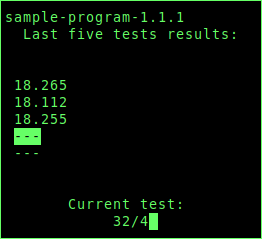
\includegraphics[scale=2.0]{images/parameter-test.png}
\caption{Parameter-test program utolsó eredmények}
\label{fig:parameter-test}
\end{figure}

Végül a menu ablakot törli és újrarajzolja a következő iterációban.
Amikor a teszt végzett, az összes kernel változó végigpróbálásával, a fájlt lezárja és visszaállítja a változókat az eredeti értékükre.
Az így kapott fájl formátuma json típusú, ez főként a feldolgozás miatt volt fontos.
\Section{SchedulerTuneML program}
A program Python programozási nyelven készült, több különböző modul felhasználásával.
 A program célja hogy, parameter-test program által készített json fájlokat feldolgozza. A fájlból kinyert adatokat elemezni, besorolja őket csoportokba, diagrammokat készít ezekről és javaslatokat tesz a kernel változók értékeinek beállítására, az adott felhasználási módhoz viszonyítva.

\SubSection{SchedulerTuneML program implentációja }
A program Jupyter Notebook-ban készült, emiatt a fájlok .ipynb kiterjesztésüek. Kihasználva a notebook által készíthető cellákat, a legtöbb kódrészlet mellé készítettem leírásokat, úgy gondolom hogy egyszerűbben megérthetők ezekkel, az egyes kódrészletek.
%a programokat kategóriákba sorolom
A benchmark program által készített eredmények tesztenként eltérőek, ami főként a különböző felhasználási módból következik. Ezeket az értékeket normalizálnom kell először, mielőtt felhasználnám a model betanításánál. Ehhez feature scaling-et alkalmaztam, ami azt jelenti hogy abban az esetben amikor a teszt értékek közül a kisebb érték számít jobbnak a következő képletet használom fel. 
\begin{equation}
x = \frac{max-x}{max-min}
\end{equation}
Amennyiben a nagyobb érték számít jobbnak, az előző képlett kicsit módosított változatát.
\begin{equation}
x = \frac{x-min}{max-min}
\end{equation}
Ezek felhasználásával, biztosítom hogy az értékek nulla és egy között maradjanak.
A meglévő adathalmazom azonban önmagában nem elegendő arra hogy, a neurális hálót be tudjam tanítani vele, emiatt új elemeket, illetve kategóriákat vezettem be.
\begin{itemize}
\item resultClass

A program első lépései, a json fájlok megnyitása, az értékeken történő végigiterálás, annak érdekében hogy megtaláljam a legkisebbet, illetve a legnagyobbat. Ezt követően létrehozok 5 szintet az értékek csoportosítására, amely a következő képpen történik.
\begin{alignat*}{2}
         x& < 20 &: 0 \\
    20 < x& < 40 &: 1 \\
    40 < x& < 60 &: 2 \\
    60 < x& < 80 &: 3 \\
    80 < x& < 100&: 4
\end{alignat*}

\item serverWorkload

A Linux kernel dokumentációjában olvashatunk az ütemezőt behangolhatjuk, szerver szintű terhelésre. Ezt az eredményt, a sched\_min\_granularity\_ns kernel változó módosításával érhetjük el.
Mivel a szerver szintű terheléseknél, sűrűbben fordulnak elő batch processzek, azaz akik életük nagyrészét inkább számításokkal töltik és náluk előnyösebb nagyobb időszeleteket használni. Ezt az eredményt pedig elérhetjük ennek a változó módosításával. Így amikor nagyobb értéket vesz fel a sched\_min\_granularity\_ns mint az alapbeállítás, serverWorkload kategóriába kerül.
\item swap 

A swap csoport gyakorlatilag a swap memória igényt jelzi. 
Minden olyan mérési eredményt, amelynél nem fordult elő swap memória használat, nullával láttam el, ellenkező esetben pedig eggyessel.
\item batchProcess

Batch processzek, nem szükséges nagy prioritást állítani, kevesebbszer kerülnek végrehajtásra, viszont ekkor nagyobb időszeletet is kaphatnak. Emiatt hogyha egy processz prioritása nagyobb mint nulla, batchProcess kategóriába kerül.
\end{itemize}

A felsorolt kategóriák, fontos részét képezik az adathalmaznak amit kialakítottam. Ebbe az adathalmazba szintén beletartoznak a benchmarkokból származó eredmények, amik átestek a feature scaling-en, illetve a hozzá tartozó kernel változók. Az adathalmazból egy DataFrame-et készítettem, a Pandas modul segítségével. Ezáltal egyszerűen átláthatom, lekérdezhezhetek belőle részeket, és ábrázolhatom az adatokat.
Az így kapott DataFrame segítségével fogom megkísérelni egy neurális hálózat betanítását. 
%TODO referencia könyvből: Hands-On Machine Learning with Scikit-Learn, Keras, and TensorFlow: Concepts, Tools, and Techniques to Build Intelligent Systems 2nd Edition
A gépi tanulásra találtam egy rövid definíció, az egyik könyvben:

\begin{quote}
``A gépi tanulás az a tanulmányi terület, amely képessé teszi a számítógépeket a tanulásra
anélkül, hogy kifejezetten beprogramozták volna.''
\par\nobreak\smallskip\hfill—Arthur Samuel, 1959
\end{quote}

A gépi tanulásnál számos területe létezik, azonban az én problémám megoldására supervised learning-et alkalmaztam. Ami azt jelenti hogy, az adathalmazban az egyes mintáknál, megtalálhatók a tulajdonságok(features), illetve az elvárt eredmények is(labels).
Mivel a kernel változók intervallumait négy részre szedtem szét a teszteléseknél, így erre egy klasszifikációs algoritmust használok fel.
A modelt az adott problémához mérten kell felépíteni, amihez fontos hogy optimálisan válasszuk meg rejtett rétegek, illetve a neuronok számát.
Az én esetemben, a model öt bemenettel, illetve öt kimenettel rendelkezik és egy rejtett réteget választottam a feladathoz.

\begin{figure}[h!]
\centering
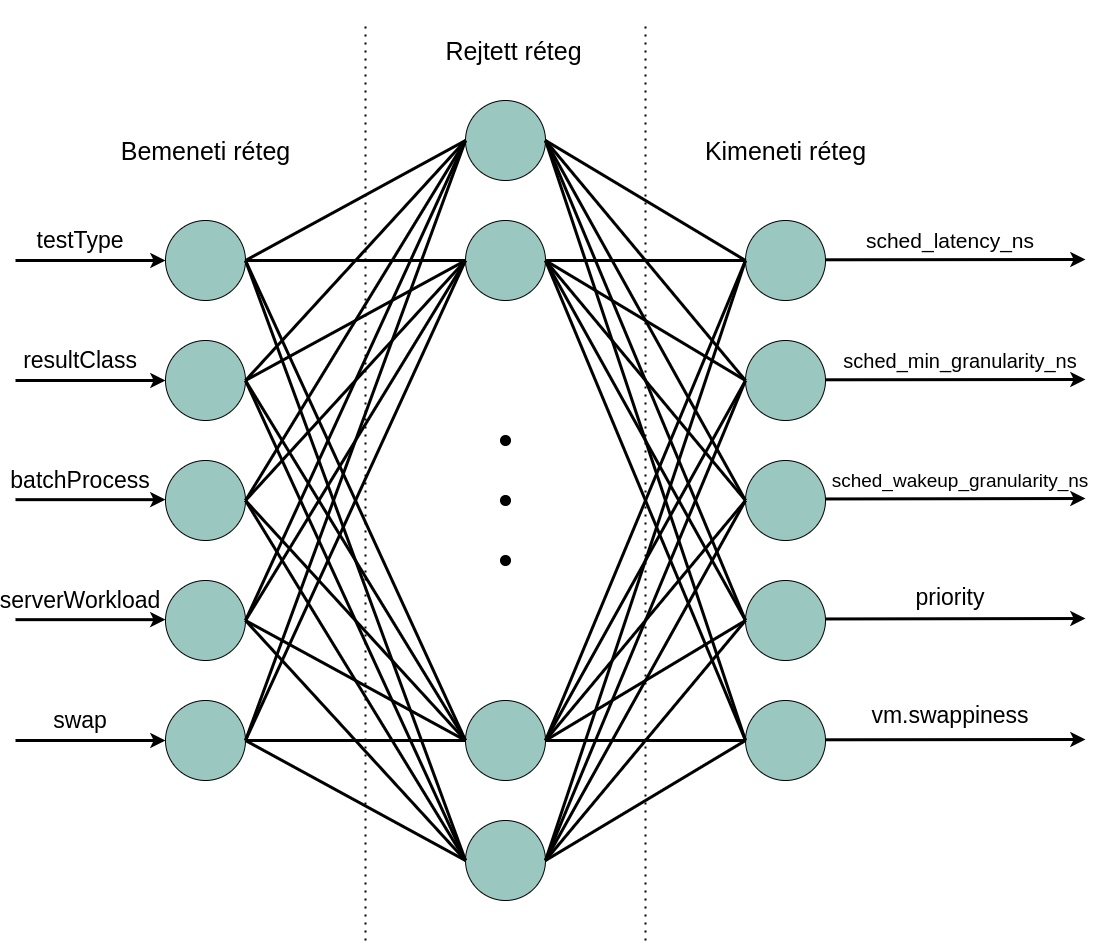
\includegraphics[scale=0.3]{images/neuralNetwork.png}
\caption{Neurális hálózat}
\label{fig:neuralnetwork}
\end{figure}

Alapvetően ezek a mesterséges neuronok, fogalmilag biológiai idegsejtekből származnak.
Minden neuron több bemenettel rendelkezik és egyetlen kimenettel amit több neuronnak is képes továbbítani.

\noindent A neuron által kiszámított kimeneti érték, a következő képpen kapható meg.
\begin{figure}[h!]
\centering
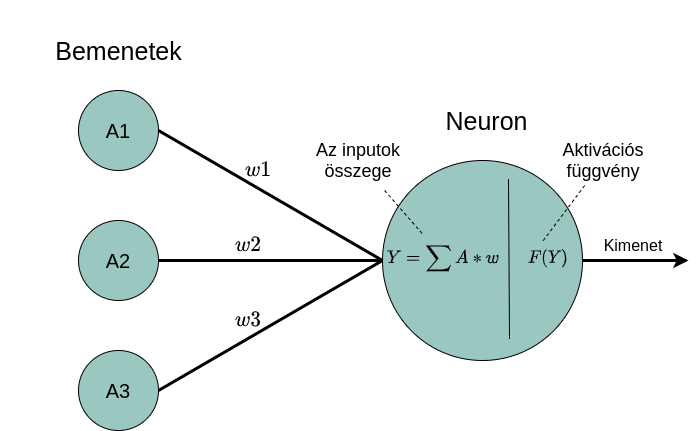
\includegraphics[scale=0.3]{images/neuron.png}
\caption{Neuron}
\label{fig:neuron}
\end{figure}

Az inputokat beszorozzuk a hozzájuk tartozó súlyokkal, majd ezeket összeadjuk és az így kapott értéket behelyettesítjük az aktivációs függvénybe.
%TODO referencia: https://towardsdatascience.com/activation-functions-neural-networks-1cbd9f8d91d6
Az aktivációs függvénnyel elérhetjük hogy az érték 0 és 1 között maradjon, vagy néhány esetben -1 és 1 között (függvénytől függ). Ezzel határozzuk meg a neurális hálózat kimenetét, olyan mint hogyha azt mondanánk hogy igen vagy nem. (Történik aktiváció vagy sem.) 
A következő aktivációs függvények közül választhatunk, az sklearn Klasszifikációs algoritmusához.
\begin{itemize}
\item identity - $f(x) = x$

Egy egyszerű lineáris függvény, értékkészlete $\mathbb{R}$.
\item logistic - $f(x) = \frac{1}{1+e^{-x}}$

Logisztikus vagy Szigmoid függvény, ami eg S alakot ír le. Az oka amiért előszeretettel használjuk ezt a függvényt az hogy, az értékkészlete pont 0 és 1 között található. Ez különösen azoknál a modelleknél alkalmazzák, ahol a valószínűséget kimenetként kell megjósolnunk.
\item tanh - $f(x) = \frac{e^{x}-e^{-x}}{e^{x}+e^{-x}}$

A tangens hiperbólikusz függvény nagyon hasonló a szigmoidhoz, de jobb nála. Az értékkészlete -1-től 1-ig tart, és ő is S alakú függvény.
A negatív részének nagy előnye van, mivel ezt vehetjük úgymond erősen negatívnak, azaz egy erős "nem" kimenetnek. Jellemzően klasszifikációs modelleknél használják ezt a függvényt.
\item relu (Rectified Linear Unit) - $f(x) = max(0,x)$

A ReLU jelenleg a világon a leggyakrabban használt aktivációs függvény.
Az $f(x)$ függvény értéke nullát vesz fel, minden olyan esetben amikor $x$ értéke nulla vagy kisebb mint nulla és $f(x)$ értéke megegyezik $x$ értékével, ha $x$ nagyobb mint nulla.
A függvény értékkészlete $[0,\infty)$.
\end{itemize}

Amennyiben az adott modelben több rejtett réteg is található, az előző aktivációs függvény érték veszi fel a bemeneti érték szerepét és így halad tovább az algoritmus. Amikor sikeresen elértünk az kimeneti réteghez, a kapott eredményt összehasonlítjuk az elvárttal, ebből egy hibát számítunk.
Ekkor visszafele haladunk a modelben és a kapott hibával újraszámítjuk a súlyokat.
Ezután pedig ismételten előre iterálunk, az új súly értékeket felhasználva a neuron számításoknál.

A rejtett rétegben elhelyezkedő neuronok számának meghatározásához nincs semmiféle varázsképlet, azonban találtam néhány ökölszabályt, amik a következők. 
%TODO referencia könyvből: Introduction to Neural Networks with Java: page 129
\begin{itemize}
\item A rejtett rétegben lévő neuronok száma, a bemeneti és kimeneti rétegek méretei között kell hogy essenek.
\item A rejtett rétegben lévő neuronok száma, legyen a bemeneti réteg méretének kétharmada, amihez hozzáadjuk a kimeneti réteg méretét.
\item A rejtett rétegben lévő neuronok száma, legyen kevesebb mint a bemeneti réteg méretének a kétszerese.
\end{itemize}

%TODO referencia az sklearn oldaláról: https://scikit-learn.org/stable/modules/generated/sklearn.neural_network.MLPClassifier.html
Gépi tanulás algoritmusai gyakran támaszkodnak valamilyen célfüggvény optimalizálásra, ezért az optimalizálási algoritmus megválasztása a tanulás folyamat egyik fontos része.
Az sklearn.neural\_network.MLPClassifier esetén, három választásunk van.
\begin{itemize}
\item ADAM, ami egy sztochasztikus gradiens alapú optimalizáló algoritmusra utal, amelyet még Kingma, Diederik és Jimmy Ba javasolt.
\item sgd (stochastic gradient descent), amely a negatív gradiens irányába tesz lépéseket a célfüggvényhez.
\item L-BFGS, egy  optimalizáló algoritmus a kvázi Newton-módszerek családjából.

\end{itemize}

A rejtett réteghez tartozó neuron szám, aktivációs függvény és solver megválasztásához egy grid search technikát alkalmazok.
%referencia az sklearn GridSearch és Cross Validation-re: https://scikit-learn.org/stable/modules/cross_validation.html
\begin{figure}[h!]
\centering
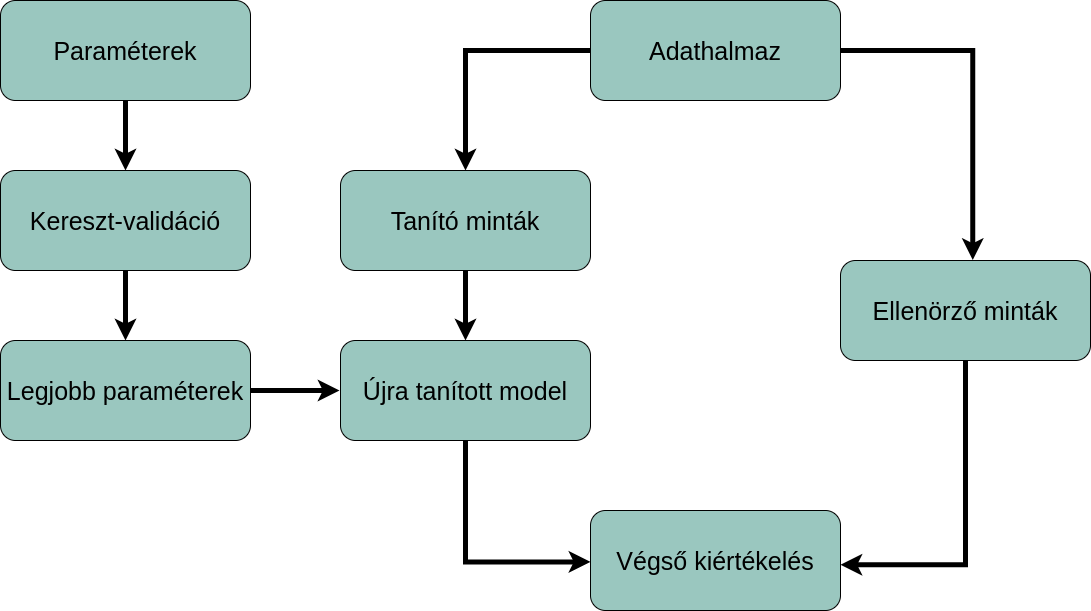
\includegraphics[scale=0.3]{images/gridSearch.png}
\caption{Kereszt-validáció, a paraméterek megkeresésére}
\label{fig:neuralnetwork}
\end{figure}

Erre az sklearn.grid\_search.GridSearchCV függvényt választottam, ami egy kimerítő keresést végez, a legjobb paraméterek megtalálásához. A függvény alkalmazásához készítenem kellett egy paraméter készletet, amiben végig próbálja az összes lehetséges kombinációját. Ami azt jelenti hogy, minden próba végén kiértékeli a modelt egy Cross-Validation módszer segítségével. Ezáltal megkaptam azokat a model paramétereket, amivel a legjobban teljesített.
A modelhez így a tangens hiperbólikusz használtam fel aktivációs függvényként, emellett kilenc rejtett rétegben található neuron és az L-BFGS optimalizáló algoritmust alkalmaztam.

%TODO referencia könyvből: Hands-On Machine Learning with Scikit-Learn and TensorFlow
Az egyetlen módja hogy kiderítsem hogyan teljesít a model, ki kell hogy próbáljam új adatokkal. 
Ezt megtehetem úgy hogy késznek nyilvánítom a programot tanítás után és a felhasználók amikor majd kipróbálják, kiderül hogy sikerült. Ez az ötlet ugyan müködhet, de amennyiben a model rosszul lett felépítve meglehet hogy nagyon rosszul teljesít és a felhasználóknak nem fogja elnyerni a tetszésüket. Egy okosabb módszer a rendelkezésre álló adathalmazt, szétszedni két részre. Az első halmazban találhatók a tanító minták, amikkel a model betanítását fogom végezni. A második halmaz pedig az ellenörzésre szolgál, itt a mintákkal csak tesztelem a model teljesítményét.
Ezeket training és testing set-nek is szokás nevezni, az utóbbi felhasználásával kiderülhet a hibaarány mérete, amit szokás általánosítási hibának is nevezni. Ez az érték megmondja, hogy a model mennyire fog jól teljesíteni olyan mintákon, amelyeket még nem látott korábban.
Amennyiben a model rosszul teljesített a tanító és az ellenörző mintákat tartalmazó adathalmazon egyaránt, fennállhat az alul tanulás problémája, erre egy megoldás lehet az hogyha komplexebb modelt tervezünk. Abban az esetben ha jól teljesített a tanító mintákon, viszont rosszul az eddig még nem látottakon, előfordulhat hogy a model túl tanult. A cél a kettő között helyezkedik el, így erre nagy figyelmet kell model készítés során.
Gyakori, hogy az adatok 80\% -át használják fel tanításra, és a maradék 20\% -ot tesztelésre. Ez azonban az adatkészlet méretétől függ, amennyiben az adathalmazunk 10 millió példányt tartalmaz, elég lehet az adatok 1\% -át felhasználni tesztelésre, 100 000 példány valószínűleg több, mint
elég ahhoz, hogy jó becslést kapjunk az általánosítási hibáról. Az én esetemben az adathalmazomban 6144 minta található, emiatt én az adatok 80\%-át fogom felhasználni tanításra és a maradékot pedig a model tesztelésére fordítom. Erre a célra én az sklearn.model\_selection.train\_test\_split függvényt fogom felhasználni. 

\begin{python}
X = df[["testType","resultClass","batchProcess","serverWorkload","swap"]]
y = df[["latency","min_gran","wakeup_gran","priority","vm.swappiness"]]
X_train,X_test,y_train,y_test = train_test_split(X,y,test_size=0.2)
\end{python}

Paraméterként meg kell adjam a használati módokat(X), a hozzátartozó kernel változókat(y) és az tesztelési adathalmaz méretét \%-os formában.
Az X változó gyakorlatilag egy részlet a dataFrame-ből, ami látható a következő kódrészletből.

A testType az adott felhasználási módot jelöli, az elérhető felhasználási módok a benchmark kategória típusok. Az elérhető kategóriák a következők: 
\begin{enumerate}
\item Egy CPU magot igénylő, processzor igényes felhasználási mód.
\item Több CPU magot igénylő, magas processzor intenzitású felhasználási mód.
\item Rendszert terhelő felhasználási mód.(Sok rendszerhívásra lehet számítani)
\item Háttértárat terhelő felhasználási mód.
\item Memóriát és processzort terhelő felhasználási mód.
\item Videókártyát terhelő felhasználási mód.
\end{enumerate}

A resultClass az eredmény besorolása, kategóriákba. Ezt az értéket mindig 4-re állítom, ezzel próbálom meg elérni hogy mindig a legjobb értékek közül kapjak paramétereket.

A batchProcess paraméter segítségével beállítható hogy az adott processzt kívánja-e a felhasználó batch módban futtatni. Ez a processz prioritását és a processzhez tartozó vruntime változó értékének módosítását jelenti. A batchProcess mód beállításhoz 1-re kell állítani a változó értékét, egyébként 0-ra.

A serverWorkload segítségével a felhasználó a futtatni kívánt processzeihez mérten beszabályozhatja az ütemezőt. Amennyiben a processzek amiket futtatni szeretne, szerver szintű terhelési módhoz állnak közel, érdemes ezt a változót 1-re állítani, ellenkező esetben 0-ra.

A swap paraméterrel, a felhasználó eldöntheti hogy szeretne-e swap memóriát használni. Érdemes lehet ezt a változót beállítani 1-re, kevés memóriával rendelkező számítógépek esetén. Abban az esetben ha nincs szüksége erre az opcióra, 0-ra kell beállítania az értéket.

A kimenet a paraméterkészlet az ütemező hangoláshoz, a futtatni kívánt processzekhez az ajánlott prioritás és swap memóriát szabályzó kernel paraméter, az adott felhasználási módhoz mérten.
A model létrehozása és betanítása a következő képpen történik az sklearn library felhasználásával. 
\begin{python}
model = MultiOutputClassifier(MLPClassifier(
	solver="lbfgs",
	hidden_layer_sizes=(9,),
	activation="tanh"))
model.fit(X_train,y_train)
\end{python}
A hagyományos model létrehozása során elég csak az MLPClassifier-t meghívni, a kívánt paraméterekkel. Az én esetem viszont kicsit máshogy néz ki, a modellem több bemenettel, illetve kimenetettel rendelkezik. A MultiOutputClassifier ezt valósítja meg nekem, és paraméterként pedig egy estimator-t vár, ami jelen esetben nálam az MLPClassifier.

%TODO referencia a joblib-hez: https://scikit-learn.org/stable/modules/model_persistence.html
Annak érdekében hogy tesztelés gördülékenyebben zajlódjon, a modelt előre betanítottam, így futtatáskor nincs szükség újra és újra elvégezni a tanítást.
A model lementéséhez, többféle lehetőség is rendelkezésre áll. Én ehhez a joblib modult választottam, mivel sokkal effektívebb olyan objektumoknál amik nagyobb méretű numpy tömböket tartalmaznak és a sklearn oldalán is ennek a használatát javasolják.
Két függvényt alkalmazok, az első a lementést valósítja meg joblib.dump(), ami paraméterként az elkészített modelt kapja meg és hogy milyen néven mentsük el.
A másik a betöltésért felel, itt egyszerűen csak a fájlnévre hivatkozunk.
Mint ahogy látható az alábbi kódrészletből, szintaktikailag sem mondható túl bonyolultnak.

\begin{python}
joblib.dump(model,"model.sav") 
model = joblib.load("model.sav") 
\end{python}
A model, a teszt eredmények és az elkészült programok, mind megtalálhatók github-on

